The simulation results using Modelica is presented as follows: \\
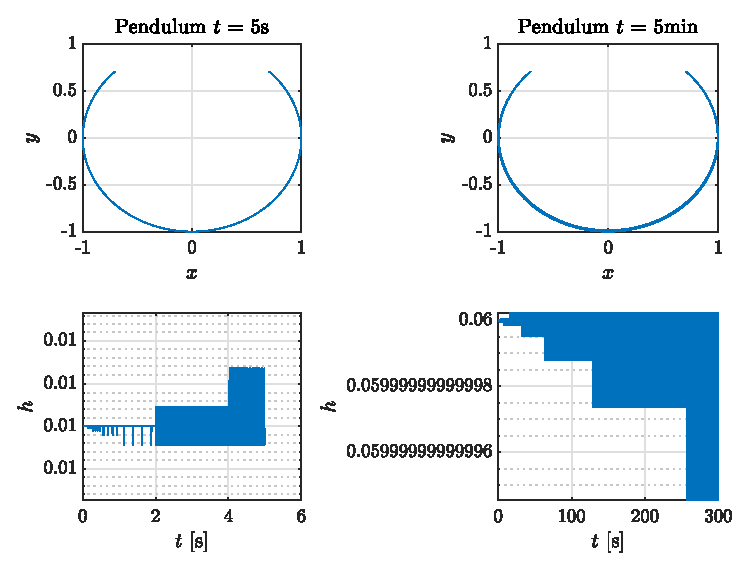
\includegraphics[width=\textwidth]{Figures/Ugf2_29.eps}
The code is as follows:
\begin{lstlisting}
	model Pendulum
		constant pi=3.14
		parameter Real phi0 = 45*pi/180;
		parameter Real L = 1, M = 1, g=9.82;

		Real x(start=L*cos(phi0)), dx(start=0);
		Real y(start=L*sin(phi0)), dy(start=0);
		Real lambda;
	equation
		der(x) = dx;
		der(y) = dy;
		M*der(dx) = lambda*x;
		M*der(dy) = lambda*y-M*g;
		0 = x*x+y*y-L*L;
	end Pendulum;
\end{lstlisting}